\documentclass[a4paper,12pt]{article}
\usepackage{ amssymb }
\usepackage{mathtools}
\usepackage{listings}
\usepackage{color}
\usepackage[utf8]{inputenc}
\DeclarePairedDelimiter\ceil{\lceil}{\rceil}
\DeclarePairedDelimiter\floor{\lfloor}{\rfloor}

\definecolor{codegreen}{rgb}{0,0.6,0}
\definecolor{codegray}{rgb}{0.5,0.5,0.5}
\definecolor{codepurple}{rgb}{0.58,0,0.82}
\definecolor{backcolour}{rgb}{0.95,0.95,0.92}
\definecolor{highlightcolor}{rgb}{0.8, 0.9, 0.9}

\usepackage{graphicx}
\graphicspath{{/Users/psholtz/Documents/Probability/}}

\newcommand{\quotes}[1]{``#1''}

\lstdefinestyle{mystyle}{
    backgroundcolor=\color{backcolour},   
    commentstyle=\color{codegreen},
    keywordstyle=\color{magenta},
    numberstyle=\tiny\color{codegray},
    stringstyle=\color{codepurple},
    basicstyle=\footnotesize,
    breakatwhitespace=false,         
    breaklines=true,                 
    captionpos=b,                    
    keepspaces=true,                 
    numbers=left,                    
    numbersep=5pt,                  
    showspaces=false,                
    showstringspaces=false,
    showtabs=false,                  
    tabsize=2
}
 
\lstset{style=mystyle}

\newcommand*\Suppressnumber{%
  \lst@AddToHook{OnNewLine}{%
    \let\thelstnumber\relax%
     \advance\c@lstnumber-\@ne\relax%
    }%
}

\begin{document}

\noindent{
\framebox {
\begin{minipage}{\dimexpr\textwidth-2\fboxsep-2\fboxrule\relax}
\vspace{2mm}
1.  (a) How many different 7-place license plates are possible if the first 2 places are for letters and the other 5 for numbers?

(b) Repeat part (a) under the assumption that no letter or number can be repeated in a single license plate. 
\vspace{2mm}
\end{minipage}
}
}

\vspace{2mm}
For part (a), we have $N = 26 \cdot 26 \cdot 10^5 = 67,600,000$.

\vspace{2mm}
For part (b), we have $N = 26 \cdot 25 \cdot 10 \cdot  9 \cdot 8 \cdot 7 \cdot 6 = 19,656,000$.

\vspace{4mm}
\noindent{
\framebox {
\begin{minipage}{\dimexpr\textwidth-2\fboxsep-2\fboxrule\relax}
\vspace{2mm}
2. How many outcome sequences are possible when a die is rolled four times, where we say, for instance, that the outcome is 3, 4, 3, 1 if the first roll landed on 3, the second on 4, the third on 3, and the fourth on 1?
\vspace{2mm}
\end{minipage}
}
}

\vspace{2mm}
We have $N = 6^4 = 1,296$.

\vspace{4mm}
\noindent{
\framebox {
\begin{minipage}{\dimexpr\textwidth-2\fboxsep-2\fboxrule\relax}
\vspace{2mm}
3. Twenty workers are to be assigned to 20 different jobs, one to each job. How many different assignments are possible? 
\vspace{2mm}
\end{minipage}
}
}

\vspace{2mm}
We have $N = 20! = 127,058,998,962,946,048$

\vspace{4mm}
\noindent{
\framebox {
\begin{minipage}{\dimexpr\textwidth-2\fboxsep-2\fboxrule\relax}
\vspace{2mm}
4. John, Jim, Jay and Jack have formed a band consisting of 4 instruments. If each of the boys can play all 4 instruments, how many different arrangements are possible? What if John and Jim can play all 4 instruments, but Jay and Jack can each play only piano and drums?
\vspace{2mm}
\end{minipage}
}
}

\vspace{2mm}
If all four boys can play all four instruments, we have $N = 4! = 24$.

\vspace{2mm}
If John and Jim can play all four instruments, but Jay and Jack can each play only piano and drums, we have $N = 2 \cdot 1 \cdot 2 \cdot 1 = 4$.

\vspace{4mm}
\noindent{
\framebox {
\begin{minipage}{\dimexpr\textwidth-2\fboxsep-2\fboxrule\relax}
\vspace{2mm}
5. For years, telephone area codes in the United States and Canada consisted of a sequence of three digits. The first digit was an integer between 2 and 9, the second digit was either 0 or 1, and the third digit was any integer from 1 to 9. How many area codes were possible? How many area codes starting with a 4 were possible? 
\vspace{2mm}
\end{minipage}
}
}

\vspace{2mm}
With no restrictions, the number of area codes is $N = 8 \cdot 2 \cdot 9 = 144$.

\vspace{2mm}
The number of area codes that start with a 4 are $N = 1 \cdot 2 \cdot 9 = 18$.

\noindent{
\framebox {
\begin{minipage}{\dimexpr\textwidth-2\fboxsep-2\fboxrule\relax}
\vspace{2mm}
6. A well-known nursery rhyme starts as follows: 

\vspace{2mm}
\hspace{2mm}``As I was going to St. Ives

\hspace{2mm}I met a man with 7 wives

\hspace{2mm}Each wife had 7 sacks.

\hspace{2mm}Each sack had 7 cats.

\hspace{2mm}Each cat had 7 kittens..."

\vspace{2mm}
How many kittens did the traveler meet?
\vspace{2mm}
\end{minipage}
}
}

\vspace{2mm}
We have $N = 7^4 = 2,401$.

\vspace{4mm}
\noindent{
\framebox {
\begin{minipage}{\dimexpr\textwidth-2\fboxsep-2\fboxrule\relax}
\vspace{2mm}
7. (a) In how many ways can 3 boys and 3 girls sit in a row?

(b) In how many ways can 3 boys and 3 girls sit in a row if the boys and the girls are each to sit together?

(c) In how many ways if only the boys must sit together?

(d) In how many ways if no two people of the same sex are allowed to sit together? 
\vspace{2mm}
\end{minipage}
}
}

\vspace{2mm}
For part (a), we have $N = (3+3)! = 6! = 720$.

\vspace{2mm}
For part (b), there are $3!=6$ ways to order 3 boys, and there are $3!=6$ ways to order 3 girls. There are $2! = 2$ ways to order a set with two elements (i.e., boys and girls being the two elements). Hence we have $N = 6 \cdot 6 \cdot 2 = 72$.

\vspace{2mm}
For part (c), there are $3!=6$ ways to order 3 boys, and there are $4!=24$ ways to order a set with four elements (the four elements being a group of boys along with three girls). Hence we have $N = 6 \cdot 24 = 144$.

\vspace{2mm}
For part (d), if we start the row with a boy, there are 3 ways to pick the seat. Similarly, there are 3 ways to pick the next seat where a girl will sit, and 2 way to pick the third seat where the next boy will sit, and 2 ways to pick the fourth seat where the second girl will sit. The choices for the final two seats are now fixed. The final result will be twice this value, since we could have begun the row with a girl as well. The final result is $N = 2 \cdot 3 \cdot 3 \cdot 2 \cdot 2 = 72$.

\pagebreak
\noindent{
\framebox {
\begin{minipage}{\dimexpr\textwidth-2\fboxsep-2\fboxrule\relax}
\vspace{2mm}
8. How many different letter arrangements can be made from the letters

(a) Fluke?

(b) Propose?

(c) Mississippi?

(d) Arrange?

\vspace{2mm}
\end{minipage}
}
}

\vspace{2mm}
For part (a), ``fluke", we have 5 unique letters, so $N = 5! = 120$.

\vspace{2mm}
For part (b), ``propose", we have 7 letters total, with the letter ``p" repeating 2 times and the letter ``o" repeating 2 times, so $N = 7! / (2! \cdot 2!) = 1,260$.

\vspace{2mm}
For part (c), ``mississippi", we have 11 letters total, with the letter ``s" repeating 4 times, the letter ``i" repeating 4 times and the letter ``p" repeating 2 times. Hence, $N = 11!/(4! \cdot 4! \cdot 2!) = 34,650$.

\vspace{2mm}
For part (d), ``arrange", we have 7 letters total, with the letter ``a" repeating 2 times and the letter ``r" repeating 2 times, so $N = 7!/(2! \cdot 2!) = 1,260$.

\vspace{4mm}
\noindent{
\framebox {
\begin{minipage}{\dimexpr\textwidth-2\fboxsep-2\fboxrule\relax}
\vspace{2mm}
9. A child has 12 blocks, of which 6 are black, 4 are red, 1 is white and 1 is blue. If the child puts the blocks in a line, how many arrangements are possible?
\vspace{2mm}
\end{minipage}
}
}

\vspace{2mm}
The number of arrangements is given by $N = 12!/(6! \cdot 4! \cdot 1! \cdot 1!) = 27,720$.

\vspace{4mm}
\noindent{
\framebox {
\begin{minipage}{\dimexpr\textwidth-2\fboxsep-2\fboxrule\relax}
\vspace{2mm}
10. In how many ways can 8 people be seated in a row if

(a) there are no restrictions on the seating arrangement?

(b) persons $A$ and $B$ must sit next to each other?

(c) there are 4 men and 4 women and no 2 men or 2 women can sit next to each other?

(d) there are 5 men are they must sit next to each other?

(e) there are 4 married couples and each couple must sit together? 
\vspace{2mm}
\end{minipage}
}
}

\vspace{2mm}
For part (a), with no restrictions there are $N = 8! = 40,320$ possibilities. 

\vspace{2mm}
For part (b), persons $A$ and $B$ act as a ``single" person, and there are 2 ways to arrange $A$ and $B$ next to each other. In addition, there are 6 remaining people to seat, which means the total number of ways to arrange the seating is $N = 2 \cdot 7! = 10,080$.

\vspace{2mm}
For part (c), if we start the row with a man, there will be $N_1 = (4!)^2 = 576$ ways to arrange the seating. But we could also start the row with a  woman, which means that the total number of arrangements is $N = 2 \cdot 576 = 1,152$.

\vspace{2mm}
For part (d), there are $N_1 = 5!  = 120$ ways to seat 5 men in a  row. Additionally, there are $N_2 = 4! = 24$ ways to pair the block of men with the 3 remaining women. The total number of arrangements is thus $N = 2,880$. 

\vspace{2mm}
For part (e), there are $N_1 = 4! = 24$ ways to seat the 4 couples, and each couple can be seated in 2 ways. Since there are 4 couples total, the total number of pairs is $N = (4!) \cdot 2^4 = 384$.

\vspace{4mm}
\noindent{
\framebox {
\begin{minipage}{\dimexpr\textwidth-2\fboxsep-2\fboxrule\relax}
\vspace{2mm}
11. In how many ways can 3 novels, 2 mathematics books and 1 chemistry book be arranged on a bookshelf if

(a) the books can be arranged in any order?

(b) the mathematics books must be together and the novels must be together?

(c) the novels must be together, but the other books can be arranged in any order? 
\vspace{2mm}
\end{minipage}
}
}

\vspace{2mm}
For part (a), if there are no restrictions, the total number of arrangements is $N = 6! = 720$. 

\vspace{2mm}
For part (b), there are $N_1 = 3! = 6$ ways to arrange the novels, and $N_2 = 2! = 2$ ways to arrange the math books. Additionally, there are $N_3 = 3! = 6$ ways to arrange the groups of books, so the total number of arrangements is $N = 6 \cdot 6 \cdot 2 = 72$.

\vspace{2mm}
For part (c), there are $N_1=  3! = 6$ ways to arrange the novels, and $N_2 = 4! = 24$ ways to arrange the novels within the remaining collection of books. The total number of arrangements is $N = 6 \cdot 24 = 144$.

\vspace{4mm}
\noindent{
\framebox {
\begin{minipage}{\dimexpr\textwidth-2\fboxsep-2\fboxrule\relax}
\vspace{2mm}
12. Five separate awards (best scholarship, best leadership qualities, and so on) are to be presented to selected students from a class of 30. How many different outcomes are possible

(a) a student can receive any number of awards?

(b) each student can receive at most 1 award? 
\vspace{2mm}
\end{minipage}
}
}

\vspace{2mm}
For part (a), we have $N = 30^5 = 24,300,000$.

\vspace{2mm}
For part (b), we have $N = 30 \cdot 29 \cdot 28 \cdot 27  \cdot  26 = 17,100,720$.

\pagebreak
\noindent{
\framebox {
\begin{minipage}{\dimexpr\textwidth-2\fboxsep-2\fboxrule\relax}
\vspace{2mm}
13. Consider a group of 20 people. If everyone shakes hands with everyone else, how many handshakes take place? 
\vspace{2mm}
\end{minipage}
}
}

\vspace{2mm}
We have $N = \binom{20}{2} = 190$ handshakes. 

\vspace{4mm}
\noindent{
\framebox {
\begin{minipage}{\dimexpr\textwidth-2\fboxsep-2\fboxrule\relax}
\vspace{2mm}
14. How many 5-card poker hands are there?
\vspace{2mm}
\end{minipage}
}
}

\vspace{2mm}
Choosing 5 cards out of a deck of 52, we have $N = \binom{52}{5} = 2,598,960$.

\vspace{4mm}
\noindent{
\framebox {
\begin{minipage}{\dimexpr\textwidth-2\fboxsep-2\fboxrule\relax}
\vspace{2mm}
15. A dance class consists of 22 students, of which 10 are women and 12 are men. If 5 men and 5 women are to be chosen and then paired off, how many results are possible? 
\vspace{2mm}
\end{minipage}
}
}

\vspace{2mm}
There are $N_1 = \binom{12}{5} = 792$ ways to choose 5 men and $N_2 = \binom{10}{5} = 252$ ways to choose 5 women. Each of these sets can then be paired off in $5! = 120$ ways. The total number of combinations is thus $N = 792 \cdot 252 \cdot 120 = 23,950,080$.

\vspace{4mm}
\noindent{
\framebox {
\begin{minipage}{\dimexpr\textwidth-2\fboxsep-2\fboxrule\relax}
\vspace{2mm}
16. A student has to sell 2 books from a collection of 6 math, 7 science and 4 economics books. How many choices are possible if

(a) both books are to be on the same subject?

(b) the books are to be on different subjects? 
\vspace{2mm}
\end{minipage}
}
}

\vspace{2mm}
For part (a), we can choose 2 math books in $N_1 = \binom{6}{2} = 15$ ways, we can choose 2 science books in $N_2 = \binom{7}{2} = 21$ ways, and we can choose 2 economics books in $N_3 = \binom{4}{2} = 6$ ways. Hence there are $N = 15 + 21 + 6 = 42$ ways to sell the books. 

For part (b), there are $\binom{3}{2} = 3$ ways to choose which two subjects we will sell books from.  If we wish to sell math and science books, there are $N_1 = 6 \cdot 7 = 42$ ways to sell the books. If we wish to sell math and economics books, there are $N_2 = 6 \cdot 4 = 24$ ways to sell the books. If we wish to sell science and economics books, there $N_3=  7 \cdot 4 = 28$ ways to sell the books. Hence, there are $N = 42 + 24 + 28 = 94$ ways to sell the books. 

\pagebreak
\noindent{
\framebox {
\begin{minipage}{\dimexpr\textwidth-2\fboxsep-2\fboxrule\relax}
\vspace{2mm}
17. Seven different gifts are to be distributed among 10 children. How many distinct results are possible if no child is to receive more than one gift? 
\vspace{2mm}
\end{minipage}
}
}

\vspace{2mm}
There are $N_1 = \binom{10}{7} = 120$ ways to choose the seven children to whom the gifts will be distributed. Once these seven children are chosen, there are $N_2 = 7! = 5040$ ways to distribute the gifts among them. Hence, there is a total of $N = 120 \cdot 5040 = 604,800$ ways to distribute the gifts. 

\vspace{4mm}
\noindent{
\framebox {
\begin{minipage}{\dimexpr\textwidth-2\fboxsep-2\fboxrule\relax}
\vspace{2mm}
18. A committee of 7, consisting of 2 Republicans, 2 Democrats, and 3 Independents, is to be chosen from a group of 5 Republicans, 6 Democrats and 4 Independents. How many committees are possible? 
\vspace{2mm}
\end{minipage}
}
}

\vspace{2mm}
There are $N_1 = \binom{5}{2} = 10$ ways to choose the Republicans, $N_2 = \binom{6}{2} = 15$ ways to choose the Democrats and $N_3 = \binom{4}{3} = 4$ ways to choose the Independents. Hence, there are $N = 10 \cdot 15 \cdot 4  = 600$ ways to form the committee. 

\vspace{4mm}
\noindent{
\framebox {
\begin{minipage}{\dimexpr\textwidth-2\fboxsep-2\fboxrule\relax}
\vspace{2mm}
19. From a  group of 8 women and 6 men, a committee consisting of 3 men and 3 women is to be formed. How many different committees are possible if 

(a) 2 of the men refuse to serve together?

(b) 2 of the women refuse to serve together?

(c) 1 man and 1 woman refuse to serve together? 
\vspace{2mm}
\end{minipage}
}
}

\vspace{2mm}
Subject to no restrictions, there are $N = \binom{6}{3} \cdot \binom{8}{3} = 1,120$ ways to form the committee. 

For part (a), there are $N_1 = \binom{4}{1} = 4$ ways to choose the men where the two feuding men serve together, and there are $N_2 = \binom{8}{3} = 56$ ways to choose the women. Hence, there are $N_3 = 4 \cdot 56 = 224$ possible committees where the feuding men are serving together, and so there are $N = 1,120 - 224 = 896$ ways of selecting the committee such that the two men do not serve together. 

For part (b), there are $N_1 = \binom{6}{1} = 6$ ways to choose the women where the two feuding women serve together, and there are $N_2 = \binom{6}{3} = 20$ ways to choose the men. Hence, there are $N_3 = 6 \cdot 20 = 120$ possible committees where the feuding women are serving together, and so there are $N = 1,120 - 120 = 1,000$ ways of selecting the committee such that the two women do not serve together.  

\pagebreak
For part (c), there are $N_1 = \binom{5}{2} = 10$ ways to choose the men such that the feuding man is selected, and there are $N_2 = \binom{7}{2} = 21$ ways to choose the women such that the feuding woman is selected. Hence, there are $N_3 = 10 \cdot 21 = 210$ ways to select the committee such that the feuding man and woman are serving together, and so there are $N = 1,120 - 210 = 910$ ways to select the committee such that the feuding man and woman do not serve together. 

\vspace{4mm}
\noindent{
\framebox {
\begin{minipage}{\dimexpr\textwidth-2\fboxsep-2\fboxrule\relax}
\vspace{2mm}
20. A person has 8 friends, of whom 5 will be invited to a party.

(a) How many choices are there if 2 of the friends are feuding and will not attend together?

(b) How many choices if 2 of the friends will only attend together?
\vspace{2mm}
\end{minipage}
}
}

\vspace{2mm}
Subject to no restrictions, there are $\binom{8}{5} = 56$ ways to select the friends. 

For part (a), there are $N_1 = \binom{6}{5} = 6$ ways to choose the friends such that neither of the feuding friends is invited. There are $N_2 = \binom{6}{4} = 15$ ways to choose the friends such that only one of the feuding friends is invited, and there are 2 ways to choose this feuding friend. Hence, there are $N = 6 + 15 + 15 = 36$ ways to select the friends such that neither of the feuding friends is invited.

For part (b), there are $N_1 = \binom{6}{3} = 20$ ways to select the friends such that both friends will attend the party, and there are $N_2 = \binom{6}{5} = 6$ ways to choose the friends such that neither of the two friends is invited. Hence, there are $N = 20 +6 = 26$ ways to invite the friends such the two friends will only attend together.

\vspace{4mm}
\noindent{
\framebox {
\begin{minipage}{\dimexpr\textwidth-2\fboxsep-2\fboxrule\relax}
\vspace{2mm}
21. Consider the grid of points shown here. Suppose that, starting at the point labeled $A$, you can go one step up or one step to the right at each move. This procedure is continued until the point labeled $B$ is reached. How many different paths from $A$ to $B$ are possible? (Hint: Note that to reach $B$ from $A$, you must take 4 steps to the right and 3 steps upward). 
\vspace{2mm}
\end{minipage}
}
}

\begin{figure}[ht!]
\centering
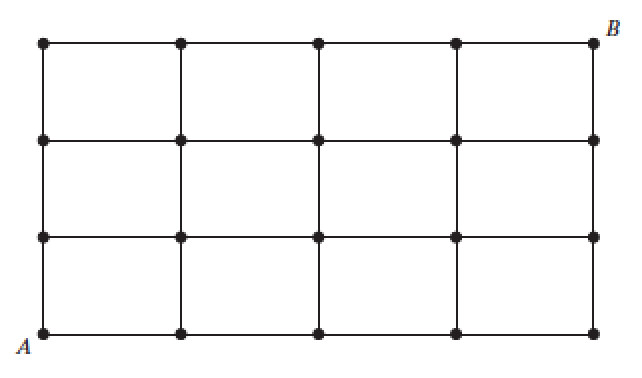
\includegraphics[width=90mm]{RossFigure001.jpg}
\end{figure}

There are a total of 7 steps in the path, 4 of the steps being horizontal and 3 of the steps being vertical. We can think of this problem as counting the number of ways to form a 7-letter word using 4 letters $H$ and 3 letters $V$ (i.e., one solution would be to go straight up, and then straight over, which would correspond to the word $VVVHHHH$).

The total number of ways to form a 7-letter word using 4 letters $H$ and 3 letters $V$ is $N = \frac{7!}{4! \cdot 3!} = 35$. Hence, there are $N = 35$ ways to reach point $B$ from point $A$. 

\pagebreak
\vspace{4mm}
\noindent{
\framebox {
\begin{minipage}{\dimexpr\textwidth-2\fboxsep-2\fboxrule\relax}
\vspace{2mm}
22. In Problem 21, how many different paths are there from $A$ to $B$ that go through the point circle in the following lattice?
\vspace{2mm}
\end{minipage}
}
}

\begin{figure}[ht!]
\centering
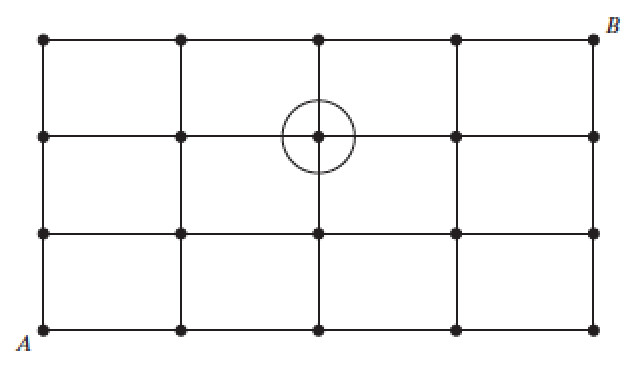
\includegraphics[width=90mm]{RossFigure002.jpg}
\end{figure}

To reach the circle point from $A$, it requires 4 steps, of which 2 are horizontal and 2 are vertical. We can think of this as counting the number of ways to form a 4-letter word using 2 letters $H$ and 2 letters $V$ (i.e., one solution would be to go straight up, and then straight over, which would correspond to the word $VVHH$).

The total number of ways to form a 4-letter word using 2 letters $H$ and 2 letters $V$ is $N = \frac{4!}{2! \cdot 2!} = 6$. Hence, the number of ways to reach the circle from point $A$ is $N_A = 6$. 

To reach the point $B$ from the circle requires 3 steps, of which 2 are horizontal and 1 is vertical. We can think of this as counting the number of ways to form a 3-letter word using 2 letters $H$ and once letter $V$. This can be done in $N_B = \frac{3!}{2! \cdot 1!} = 3$ ways. 

The total number of ways to reach point $B$ from $A$ while going through the circle is thus $N = 6 \cdot 3 = 18$.

\pagebreak
\noindent{
\framebox {
\begin{minipage}{\dimexpr\textwidth-2\fboxsep-2\fboxrule\relax}
\vspace{2mm}
23. A psychology laboratory conducting dream research contains 3 rooms, with 2 beds in each room. If 3 sets of identical twins are to be assigned to these 6 beds so that each set of twins sleeps in different beds in the same room, how many assignments are possible? 
\vspace{2mm}
\end{minipage}
}
}

\vspace{2mm}
There are $N_1 = 3! = 6$ ways to assign the twins to each room, and there are 2 ways to assign the twins within each room. Hence, the total number of assignments is $N = 3! \cdot 2^3 = 48$.

\vspace{4mm}
\noindent{
\framebox {
\begin{minipage}{\dimexpr\textwidth-2\fboxsep-2\fboxrule\relax}
\vspace{2mm}
24. Expand $(3x^2 + y)^5$.
\vspace{2mm}
\end{minipage}
}
}

From the Binomial Theorem, we have:

\[ (3x^2+ y)^5 = \sum_{j=0}^5 \binom{5}{j} (3x^2)^{5-j}y^j \]

\[ = (3x^2)^5 + 5(3x^2)^4 y +10 (3x^2)^3 y^2 + 10(3x^2)^2 y^3 + 5(3x^2) y^4 + y^5\]

\[ = 243x^{10} +  405 x^8 y + 270x^6 y^2 + 90x^4y^3 + 15x^2y^4 + y^5 \]

\vspace{4mm}
\noindent{
\framebox {
\begin{minipage}{\dimexpr\textwidth-2\fboxsep-2\fboxrule\relax}
\vspace{2mm}
25. The game of bridge is played by 4 players, each of whom is dealt 13 cards. How many bridge deals are possible?
\vspace{2mm}
\end{minipage}
}
}

The number of bridge deals is given by:

\[ N = \binom{52}{13} \cdot \binom{39}{13} \cdot  \binom{26}{13} \cdot  \binom{13}{13} \]

\[ N = \frac{52!}{39! \cdot 13!} \cdot \frac{39!}{26! \cdot13!} \cdot \frac{26!}{13! \cdot13!} \cdot \frac{13!}{0! \cdot13!} \]

\[ N = \frac{52!}{(13!)^4} \]

\pagebreak
\noindent{
\framebox {
\begin{minipage}{\dimexpr\textwidth-2\fboxsep-2\fboxrule\relax}
\vspace{2mm}
26. Expand $(x_1 + 2x_2 + 3x_3)^4$.
\vspace{2mm}
\end{minipage}
}
}

From the Multinomial Theorem, we have:

\[ (x_1 + 2x_2 + 3x_3)^4 = \binom{4}{4,0,0}x_1^4 + \binom{4}{0,4,0}(2x_2)^4 + \binom{4}{0,0,4}(3x_3)^4 \]

\[ + \binom{4}{1,3,0}x_1 (2x_2)^3 + \binom{4}{3,1,0}x_1^3 (2x_2) + \binom{4}{1,0,3}x_1(3x_3)^3 \]

\[ + \binom{4}{3,0,1}x_1^3(3x_3) + \binom{4}{0,1,3}(2x_2)(3x_3)^3 + \binom{4}{0,3,1}(2x_2)^3 (3x_3) \]

\[ +\binom{4}{2,2,0}x_1^2(2x_2)^2 + \binom{4}{2,0,2}x_1^2(3x_3)^2 + \binom{4}{0,2,2}(2x_2)^2(3x_3)^2 \]

\[ + \binom{4}{1,1,2}x_1 (2x_2) (3x_3)^2+ \binom{4}{1,2,1}x_1(2x_2)^2(3x_3) + \binom{4}{2,1,1}x_1^2(2x_2)(3x_3) \]

\vspace{2mm}
The values of the coefficients work out to $\binom{4}{4,0,0} = \binom{4}{0,4,0} = \binom{4}{0,0,4} = 1$, and $\binom{4}{1,3,0} = \binom{4}{3,1,0} = \binom{4}{1,0,3} = \binom{4}{3,0,1} = \binom{4}{0,1,3} =  \binom{4}{0,3,1} = 4$, and $\binom{4}{2,2,0} = \binom{4}{2,0,2} = \binom{4}{0,2,2} = 6$, and $\binom{4}{1,1,2} = \binom{4}{1,2,1} = \binom{4}{2,1,1} = 12$ so that:

\[ (x_1 + 2x_2 + 3x_3)^4 = x_1^4 + 16x_2^4 + 81x_3^4 \]

\[ + 32 x_1 x_2^3 + 8x_1^3x_2 + 108x_1x_3^3 \]

\[ + 12x_1^3x_3 + 216x_2x_3^3 + 96x_2^3x_3\]

\[ + 24x_1^2x_2^2 + 54x_1^2x_3^2 + 216x_2^2 x_3^2 \]

\[ +216 x_1 x_2 x_3^2 + 144x_1 x_2^2 x_3 + 72x_1^2 x_2 x_3 \]

\pagebreak
\noindent{
\framebox {
\begin{minipage}{\dimexpr\textwidth-2\fboxsep-2\fboxrule\relax}
\vspace{2mm}
27. If 12 people are to be divided into 3 committees of respective sizes 3, 4 and 5, how many divisions are possible?
\vspace{2mm}
\end{minipage}
}
}

The number of possible divisions is:

\[ N = \binom{12}{3} \binom{9}{4} \binom{5}{5} \]

\[ N = \frac{12!}{3! \cdot 9!} \cdot \frac{9!}{4! \cdot 5!} \cdot \frac{5!}{0! \cdot 5!} \]

\[ N = \frac{12!}{3! \cdot 4! \cdot 5!} = \binom{12}{3,4,5} = 27,720 \]

\vspace{4mm}
\noindent{
\framebox {
\begin{minipage}{\dimexpr\textwidth-2\fboxsep-2\fboxrule\relax}
\vspace{2mm}
28. If 8 new teachers are to be divided among 4 schools, how many divisions are possible? What if each school must receive 2 teachers?
\vspace{2mm}
\end{minipage}
}
}

For part (a), the number of divisions is:

\[ N =  \sum_{n_1 + n_2 + n_3 + n_4 = 8} \binom{8}{n_1, n_2, n_3, n_4} \]

We can use the expression:

\[ (x_1 + x_2 + ... + x_r)^n = \sum_{n_1 + ... + n_r = n}\binom{n}{n_1, ..., n_r} x_1^{n_1} \cdot \cdot \cdot x_r^{n_r} \]

\noindent
so that 

\[ (1 + 1 + ... + 1)^n = r^n = \sum_{n_1 + ... + n_r = n} \binom{n}{n_1, ..., n_r} \]

\noindent
and

\[ \sum_{n_1+n_2+n_3+n_4 = 8} \binom{8}{n_1, n_2, n_3, n_4} =  4^8 = 65,536 \]

\vspace{2mm}
For part (b), the number of divisions is:

\[ N = \binom{8}{2,2,2,2} = \frac{8!}{(2!)^4} = 2,520 \]

\noindent{
\framebox {
\begin{minipage}{\dimexpr\textwidth-2\fboxsep-2\fboxrule\relax}
\vspace{2mm}
29. Ten weight lifters are competing in a team weight-lifting contest. Of the lifters, 3 are from the United States, 4 are from Russia, 2 are from China and 1 is from Canada. If the scoring takes account of the countries that the lifters represent, but not their individual identities, how many different outcomes are possible from the point of view of scores? How many different outcomes correspond to results in which the United States has 1 competitor in the top three and 2 in the bottom three?
\vspace{2mm}
\end{minipage}
}
}

For part (a), the number of possible outcomes is:

\[ N = \binom{10}{3,4,2,1} = \frac{10!}{3! \cdot 4! \cdot 2! \cdot 1!} = 12,600 \]

\vspace{2mm}
For part (b), there are $N_1 = \binom{3}{1} = 3$ ways to choose the top-ranking American and $N_2 = \binom{7}{2} = 21$ ways to choose the remaining top-ranking contestants, which gives a total of $N_3 = 63$ ways to choose all the top-ranking contestants. 

There are also $N_1' = \binom{3}{2} = 3$ ways to choose the bottom-ranking Americans and $N_2' = \binom{5}{1} = 5$ ways to choose the remaining bottom-ranking contestants, which gives a total of $N_3' = 15$ ways to choose all the bottom-ranking contestants. 

The number of ways to choose the remaining 4 contestants in the middle is now fixed. Hence, the total number of possible outcomes is:

\[ N = 63 \cdot 15 \cdot 1 = 945 \]

\vspace{4mm}
\noindent{
\framebox {
\begin{minipage}{\dimexpr\textwidth-2\fboxsep-2\fboxrule\relax}
\vspace{2mm}
30. Delegates from 10 countries, including Russia, France, England and the United States, are to be seated in a row. How many different seating arrangements are possible if the French and English delegates are to be seated next to each other and the Russian and U.S. delegates are not to be next to each other?
\vspace{2mm}
\end{minipage}
}
}

The total number of seating arrangements, subject to no constraints, is $N_1 = 10! = 3,628,800$.

The total number of seating arrangements, where France and England sit next to each other, is $N_2 = 2 \cdot 9! = 725,760$. The number of seating arrangements, where France and England sit next to each other, and where the U.S. and Russia sit next to each other, is $N_3 = 2 \cdot 2 \cdot 8! = 161,280$. 

Hence, the number of seating arraignments here France and England sit next to each other, and where the U.S. and Russia do not sit next to each other, is:

\[ N = 2 \cdot 9! - 2 \cdot 2 \cdot 8! = 564,480 \]

\vspace{4mm}
\noindent{
\framebox {
\begin{minipage}{\dimexpr\textwidth-2\fboxsep-2\fboxrule\relax}
\vspace{2mm}
31. If 8 identical blackboards are to be divided among 4 schools, how many divisions are possible? How many if each school must receive at least 1 blackboard?
\vspace{2mm}
\end{minipage}
}
}

For part (a), we must solve the equation:

\[ n_1 + n_2 + n_3 + n_4 = 8\]

\noindent 
subject to the constraint that $n_i \ge 0$. 

The result given in the text indicates that there are $\binom{n+r-1}{r-1}$ distinct non-negative integer vectors $(x_1,...,x_r)$ satisfying the equation $\sum_{i=1}^r x_i = n$. In our case, we have $n=8$ and $r=4$, hence, the total number of solutions is:

\[ N = \binom{8+4-1}{4-1} = \binom{11}{3} = 165 \]

\vspace{2mm}
For part (b), we must solve the equation:

\[ n_1 + n_2 + n_3 + n_4 = 8\]

\noindent
subject to the constraint that $n_i > 0$.

The result given in the text indicates that there are $\binom{n-1}{r-1}$ distinct positive integer vectors $(x_1,...,x_r)$ satisfying the equation $\sum_{i=1}^r x_i = n$. In our case, we have $n=8$ and $r=4$, hence, the total number of solutions is:

\[ N = \binom{8-1}{4-1} = \binom{7}{3} = 35 \]

\vspace{4mm}
\noindent{
\framebox {
\begin{minipage}{\dimexpr\textwidth-2\fboxsep-2\fboxrule\relax}
\vspace{2mm}
32. An elevator starts at the basement with 8 people (not including the elevator operator) and discharges them all by the time it reaches the top floor, number 6. In how many ways could the operator have perceived the people leaving the elevator if all people look alike to him? What if the 8 people consisted of 5 men and 3 women and the operator could tell a man from a woman?
\vspace{2mm}
\end{minipage}
}
}

For part (a), if we indicate with $n_i$ the number of people who exit on the $i$-th floor, we can arrive at the answer by calculating how many non-negative integer solutions there are for the following equation:

\[ \sum_{i=1}^6 x_i = 8 \]

From the result in the text, there are $\binom{n+r-1}{r-1}$ distinct non-negative integer vectors $(x_1, ..., x_r)$ satisfying the equation $\sum_{x=1}^r x_i = n$. In our case, we have $n=8$ and $r=6$, so the total number of solutions is:

\[ N = \binom{8+6-1}{6-1} = \binom{13}{5} = 1,287 \]

For part (b), we must track the men and women separately. We indicate with $m_i$ the number of men who exit on the $i$-th floor, and we indicate by $w_i$ the number of women who exit on the $i$-th floor. 

A total of 5 men must exit somewhere on the 6 floors:

\[ \sum_{i=1}^6 m_i = 5 \]

\noindent
and a total of 3 women must exit somewhere on the 6 floors:

\[ \sum_{i=1}^6 w_i = 3 \]

There are $N_m = \binom{6+5-1}{6-1} = \binom{10}{5} = 252$ non-negative integer solutions to the first equation, and $N_w = \binom{6+3+1}{6-1} = \binom{8}{5} = 56$ non-negative integer solutions to the second equation. 

Any one of the combinations $(m_1,...,m_6)$ by which the men can leave the elevator can be combined with any one of the combinations $(w_1, ..., w_6)$ by which the women can leave the elevator. Hence, the total number of ways to leave the elevator that the operator can discern is:

\[ N = 252 \cdot 56 = 14,112 \]

\pagebreak
\noindent{
\framebox {
\begin{minipage}{\dimexpr\textwidth-2\fboxsep-2\fboxrule\relax}
\vspace{2mm}
33. We have 20,000 dollars that must be invested among 4 possible opportunities. Each investment must be integral in units of 1,000 dollars, and there are minimal investments that need to be made if one is to invest in these opportunities. The minimal investments are 2, 2, 3 and 4 thousand dollars. How many different investment strategies are available if:

(a) an investment is to be made in each opportunity?

(b) investments must be made in at least 3 of the four opportunities?
\vspace{2mm}
\end{minipage}
}
}

For part (a), if we invest in all 4 vehicles, we must put side $T = 2 + 2 + 3 + 4 = 11$ thousand dollars before any other decisions are made. That leaves 9 thousand dollars to invest amongst 4 different vehicles. We must therefore solve the equation:

\[ \sum_{i=1}^4 x_i = 9\]

\noindent
subject to the constraint that $x_i \ge 0$. From the result in the text, there are $N = \binom{4+9-1}{4-1} = \binom{12}{3} = 220$ ways to do this. 

For part (b), there are $\binom{4}{3} = 4$ ways to choose 3 of the 4 investment vehicles, and there is $\binom{4}{4} = 1$ ways to choose all 4 investment vehicles. 

Indicate by $V_i$ the $i$-th investment vehicle. If we choose to invest in all four investment vehicles, we have, by the previous result, $N_1 = 220$ ways to accomplish this. 

If we choose to invest only in vehicles $V_1, V_2$ and $V_3$, we must set aside $2+2+3 = 7$ thousand dollars, which leaves an additional 13 thousand dollars to be distributed amongst 3 investment vehicles: 

\[ \sum_{i=1}^3 x_i = 13 \]

\noindent
This can be done in $N_2 = \binom{3+13-1}{3-1} = \binom{15}{2} = 105$ ways. 

If we choose to invest only in vehicles $V_1, V_2$ and $V_4$, we must set aside $2+2+4 = 8$ thousand dollars, which leaves an additional 12 thousand dollars to be distributed amongst 3 investment vehicles:

\[ \sum_{x=1}^3 x_i = 12 \]

\noindent
This can be done in $N_3 = \binom{3+12-1}{3-1} = \binom{14}{2} = 91$ ways. 

If we choose to invest only in vehicles $V_1, V_3$ and $V_4$, we must set aside $2+3+4 = 9$ thousand dollars, which leaves an additional 11 thousand dollars to be distributed amongst 3 investment vehicles:

\[ \sum_{x=1}^3 x_i = 11 \]

\noindent
This can be done in $N_4 = \binom{3+11-1}{3-1} = \binom{13}{2} = 78$ ways.

If we choose to invest only in vehicles $V_2, V_3$ and $V_4$, we must set aside $2+3+4 = 9$ thousand dollars, which leaves an additional 11 thousand dollars to be distributed amongst 3 investment vehicles:

\[ \sum_{x=1}^3 x_i = 11 \]

\noindent
This can be done in $N_5 = \binom{3+11-1}{3-1} = \binom{13}{2} = 78$ ways. 

The total number of ways to make investments in at least 3 of the 4 vehicles is therefore:

\[ N = 220 + 105 + 91 + 78 + 78 = 572 \]

\end{document} 